\chapter{RESULTADOS}

\section{Diseño mecánico y de actuación}

Como resultado del proceso de diseño mecánico, se elaboró un modelo tridimensional del banco de pruebas oscilante propuesto, utilizando software de diseño asistido por computadora (CAD), específicamente Autodesk Inventor Professional. Este modelo permitió validar la disposición geométrica de los componentes, evaluar interferencias, y verificar el ensamblaje del mecanismo tipo inverted slider–crank. La estructura fue diseñada considerando criterios de rigidez, compactación y accesibilidad para la futura instalación de sensores y actuadores.

En la Figura \ref{fig:banco_vistas} se muestran las vistas del modelo CAD ensamblado. El diseño contempla un diseño propio ajustable armado desde cero, lo cual permite ajustar el recorrido sin necesidad de electrónica adicional, simplificando el prototipo y permitiendo explorar experimentalmente diferentes configuraciones de amplitud con bajo costo y alta confiabilidad mecánica.

\begin{figure}[htbp]
    \centering
    \includegraphics[width=0.48\textwidth]{images/vista1.png}
    \hfill
    \includegraphics[width=0.48\textwidth]{images/vista2.png}
    \caption{Vistas del diseño CAD del banco de pruebas oscilante}
    \label{fig:banco_vistas}
\end{figure}

Además, se realizaron vistas detalladas de componentes clave, como se observa en la Figura \ref{fig:cad_amplitud}, donde se destaca el mecanismo del actuador lineal. Esta solución permite ajustar manualmente la amplitud de oscilación, puede quedarse fija durante su uso y permite configurarla a distintas posiciones y velocidades, en este caso se está considerando una variación de 10 cm. Esta capacidad de regulación dinámica permitirá evaluar el impacto de la amplitud sobre el sistema en diferentes condiciones, facilitando la automatización de pruebas y ampliando la aplicabilidad del prototipo.

\begin{figure}[H]
\centering
\includegraphics[width=0.4\textwidth]{images/propio.png}
\caption{Detalle del mecanismo del actuador lineal}
\label{fig:cad_amplitud}
\end{figure}

%Sin embargo, también se propone emplear un actuador lineal SFU1605, %como se observa en la figura \ref{fig:act_lineal}, el cual permite %ajustar la carrera de forma precisa y programable. 

%\begin{figure}[H]
%\centering
%\includegraphics[width=0.4\textwidth]{images/3.png}
%\caption{Actuador lineal SFU1605}
%\label{fig:act_lineal}
%\end{figure}

\section{Simulación}

\subsection{Validación mediante simulación cinemática y cinética}

Con el objetivo de verificar el correcto funcionamiento del mecanismo propuesto, se realizó una simulación computacional del sistema de cinco barras tipo \textit{inverted slider-crank} utilizando un modelo dinámico basado en las ecuaciones presentadas en el Capítulo II. En la Figura~\ref{fig:sim_mechanism} se muestra la representación gráfica del mecanismo, donde se visualiza su configuración espacial y la trayectoria generada por el punto medio de del cuerpo oscilante PE. El esquema incluye todos los componentes principales del mecanismo: la manivela AB (anclada en A), la biela BC, el actuador telescópico DE (vertical, anclado en D), la corredera C sobre la plataforma PE, y el indicador de estado del actuador (MIN-MAX) en el lado derecho. Esta visualización es fundamental para verificar que el mecanismo no presenta interferencias entre componentes y opera dentro de los límites cinemáticos establecidos en el diseño, validando así el modelo antes de la construcción del prototipo físico.

\begin{figure}[H]
\begin{center}
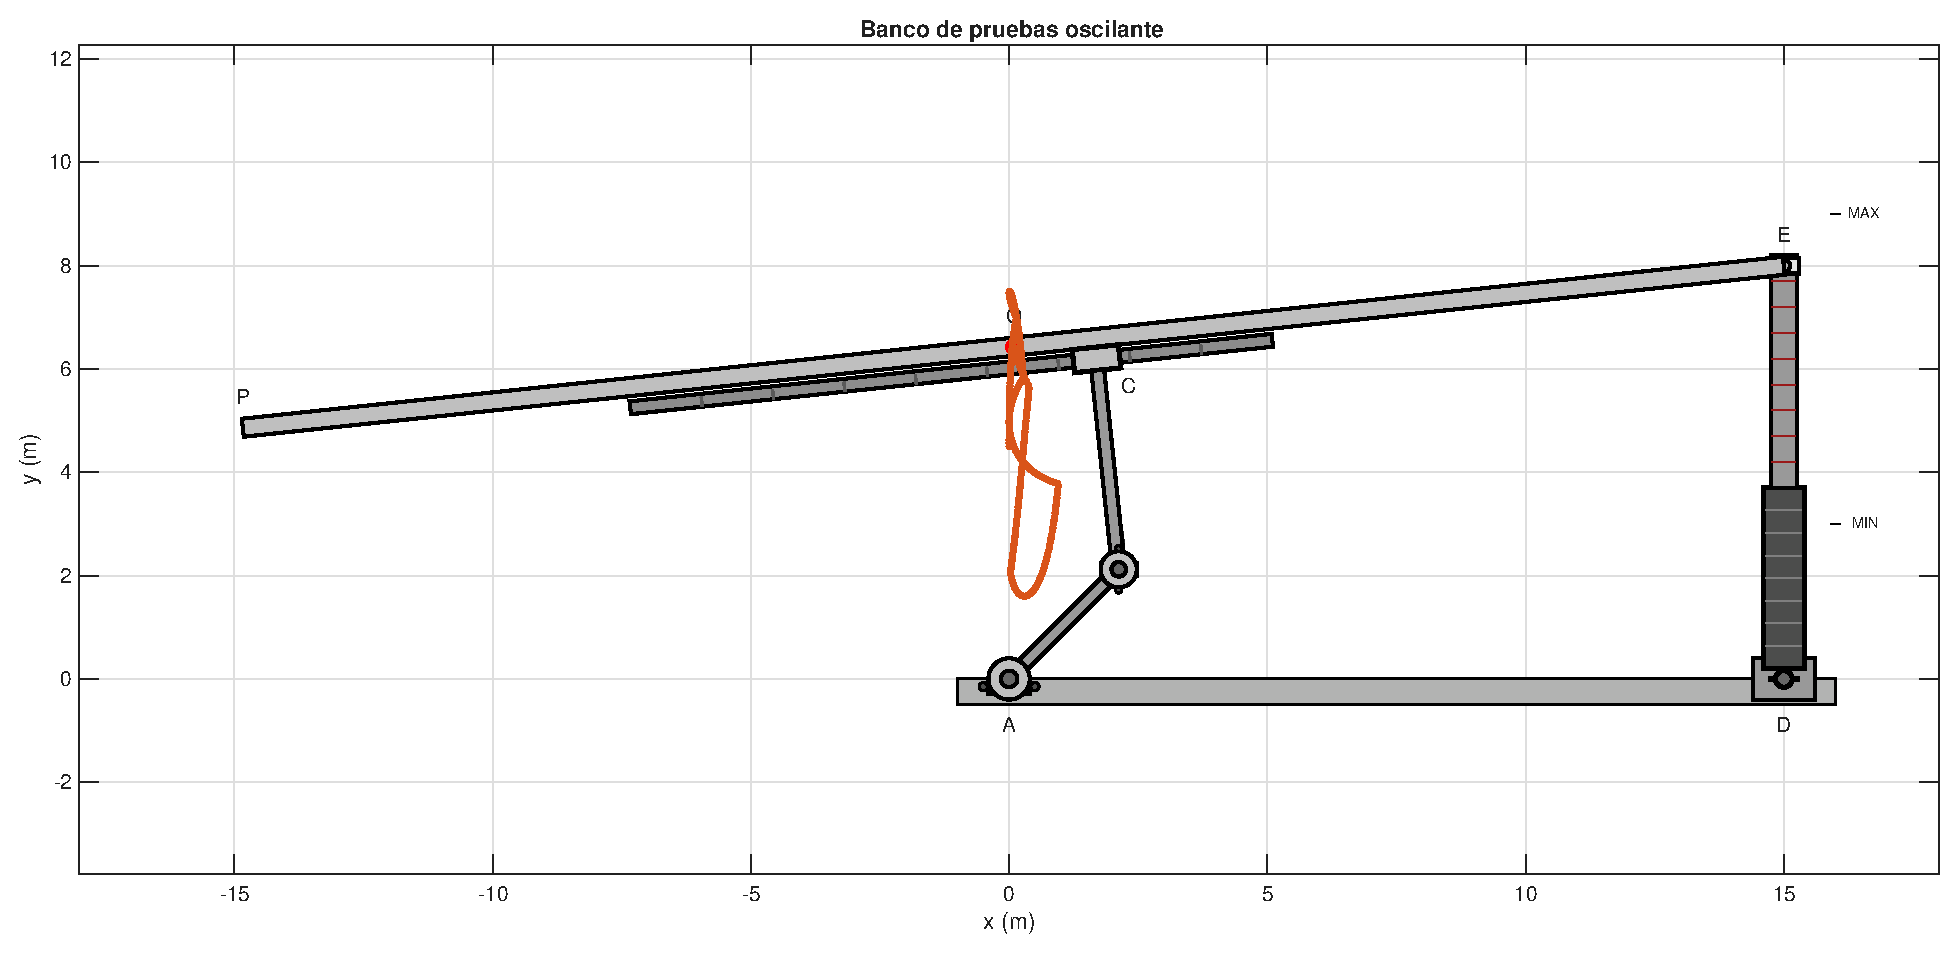
\includegraphics[width=1\textwidth]{images/sim_mechanism.eps}
\caption{Simulación del movimiento del mecanismo en MATLAB}
\label{fig:sim_mechanism}
\end{center}
\end{figure}

El modelo simulado permitió obtener las posiciones relativas de cada eslabón en función del tiempo, calculando además las velocidades y aceleraciones lineales y angulares correspondientes. La trayectoria del punto medio de la barra PE, destacada en color anaranjado, confirma el comportamiento oscilante esperado y evidencia la precisión geométrica del sistema ante diferentes posiciones de entrada.

Los resultados de la simulación coinciden con los valores teóricos obtenidos en el análisis cinemático y cinético del sistema, lo cual valida el modelo implementado y respalda la coherencia de su comportamiento dinámico. Esta correspondencia entre teoría y simulación garantiza la viabilidad del diseño propuesto para su posterior validación experimental.

A partir del modelo cinemático del mecanismo de cinco barras propuesto, se realizaron simulaciones en un entorno computacional para analizar el comportamiento del sistema bajo condiciones de entrada configurables. En esta etapa, se estudiaron cuatro variables principales: la posición angular del eslabón oscilante $\theta_4$, la posición y velocidad del punto medio $O$ de la barra $PE$, y la trayectoria completa del mecanismo durante su operación.

\begin{figure}[H]
\centering
\includegraphics[width=1\textwidth]{images/sim_theta4.eps}
\caption{Posición angular $\theta_4$ vs tiempo}
\label{fig:theta4}
\end{figure}

En la Figura~\ref{fig:theta4} se muestra la evolución de la posición angular $\theta_4$ del eslabón 4 (barra $EP$), correspondiente a la plataforma que soporta la carga. Se observa un patrón \textit{periódico complejo} con oscilaciones entre aproximadamente 163° y 206° a lo largo de 4 segundos de simulación. El comportamiento presenta variaciones de amplitud en cada ciclo, evidenciando la naturaleza no lineal del mecanismo bajo el efecto combinado del movimiento de entrada de la manivela y la acción del actuador telescópico. Los picos de aproximadamente 206° ocurren de manera periódica, con valles intermedios que alcanzan mínimos de alrededor de 164°, confirmando que el sistema genera un movimiento angular cíclico controlado que permite caracterizar el rango de oscilación de la plataforma.

\begin{figure}[H]
\centering
\includegraphics[width=1\textwidth]{images/sim_pos_o.eps}
\caption{Posición del punto $O$ vs tiempo}
\label{fig:posP}
\end{figure}

En la Figura~\ref{fig:posP} se representa la posición del punto $O$ (punto medio de la barra $PE$) en el plano cartesiano, es decir, las coordenadas $P_x (t)$ y $P_y (t)$ a lo largo del tiempo. Se observa que la \textit{coordenada vertical} $P_y$ (línea morada) oscila con amplitud considerable entre aproximadamente 1.5 m y 7.5 m, presentando un patrón sinusoidal característico que refleja el movimiento oscilante principal del sistema. En contraste, la \textit{coordenada horizontal} $P_x$ (línea azul) permanece cerca del origen con oscilaciones de menor amplitud (entre -0.2 m y 1.5 m), lo cual indica que el movimiento dominante es vertical. Los máximos de $P_y$ coinciden aproximadamente con los valores mínimos de$P_x$, revelando una correlación entre ambas componentes que define la trayectoria elíptica del punto $O$. Esta gráfica permite visualizar la trayectoria descrita por el punto medio de la barra $PE$ del mecanismo, información relevante tanto para validar la cinemática como para el posterior análisis dinámico y experimental del banco de pruebas. 

\begin{figure}[H]
\centering
\includegraphics[width=1\textwidth]{images/sim_vel_o.eps}
\caption{Velocidad del punto $O$ vs tiempo}
\label{fig:velP}
\end{figure}

La Figura~\ref{fig:velP} presenta la velocidad del punto $O$ descompuesta en sus componentes horizontal ($V_x$, línea cian) y vertical ($V_y$, línea magenta). Se aprecia que la componente vertical presenta una \textit{oscilación de mayor amplitud}, con valores que varían entre aproximadamente -15 m/s y +20 m/s, mostrando cambios bruscos de dirección que corresponden a los puntos de inversión del movimiento. La componente horizontal $V_x$ exhibe oscilaciones de menor magnitud (entre -7 m/s y +7 m/s aproximadamente), con un comportamiento más irregular debido a la configuración cinemática del mecanismo. Las discontinuidades observadas en las curvas de velocidad están relacionadas con las posiciones singulares o de cambio de configuración del sistema. Esto indica que el movimiento dominante del punto extremo es vertical, lo cual concuerda con el tipo de trayectorias generadas por la configuración tipo \textit{inverted slider-crank}. 

En conjunto, estas tres simulaciones permiten comprobar que el modelo propuesto reproduce de manera consistente el comportamiento oscilante del mecanismo, sirviendo como etapa previa de validación para el diseño mecánico, antes de su implementación física.

\section{Interfaz de Usuario Web}
Como resultado de la implementación descrita en el Marco Metodológico, se obtuvo una interfaz web completamente funcional accesible a través de WiFi desde cualquier dispositivo con navegador web. Esta interfaz constituye la herramienta principal de control y monitoreo del banco de pruebas oscilante.
\begin{figure}[H]
	\centering
	\includegraphics[width=1\textwidth]{images/interfaz.png}
	\caption{Interfaz web implementada para control del banco de pruebas oscilante}
	\label{fig:interfaz}
\end{figure}
La Figura~\ref{fig:interfaz} muestra la interfaz implementada, dividida en dos paneles principales: el generador de ondas (izquierda) y el control de motores (derecha).
\subsection{Panel Generador de Ondas}
El panel izquierdo permite crear patrones de excitación mediante la suma de componentes sinusoidales. En la configuración mostrada:
\begin{itemize}
	\item \textbf{Visualización gráfica superior}: Presenta en tiempo real las dos componentes individuales (líneas semi-transparentes) y la onda resultante (línea gruesa oscura). Un indicador vertical marca el valor instantáneo.
	\item \textbf{Componente 1} (azul): Configurada como seno con amplitud de 50 unidades y frecuencia de 1.0 Hz, se encuentra activa según indica el checkbox marcado.
	
	\item \textbf{Componente 2} (roja): Configurada como seno con amplitud de 30 unidades y frecuencia de 2.0 Hz, también activa.
	
	\item \textbf{Fórmula dinámica}: Muestra la ecuación resultante: 
	
	$y(t) = 50 \cdot \sin(1.0 \cdot t + 0°) + 30 \cdot \sin(2.0 \cdot t + 0°)$
	
	\item \textbf{Valores calculados en tiempo real}:
	\begin{itemize}
		\item Valor Y Total: 20.62 (valor instantáneo de la señal)
		\item Amplitud Máxima: 80 (suma de amplitudes activas)
		\item Tiempo: 63.97 s (contador de simulación)
		\item Componentes Activas: 2
	\end{itemize}
\end{itemize}
La interfaz permite agregar hasta 10 componentes simultáneos mediante el botón "+ Agregar", y eliminar componentes individuales según sea necesario. La velocidad de animación está configurada en 50 unidades en la captura mostrada.
\subsection{Panel Control de Motores}
El panel derecho proporciona controles independientes para ambos actuadores del sistema:
\subsubsection{Motor Rotacional}
Controla la manivela del mecanismo. En la configuración mostrada:
\begin{itemize}
	\item Velocidad: 60 RPM
	\item Dirección: Horario (CW/CCW)
	\item Indicador visual circular animado que refleja el estado actual
\end{itemize}
\subsubsection{Motor Lineal}
Controla el actuador telescópico vertical. Los parámetros visibles son:
\begin{itemize}
	\item Rango de operación: 100 mm (máximo 200 mm)
	\item Velocidad de desplazamiento: 20 mm/s (máximo 100 mm/s)
	\item Posición manual: 0 mm
	\item Modo seleccionado: Manual
	\item Barra gráfica horizontal que muestra visualmente la posición actual
\end{itemize}
Los indicadores de estado en tiempo real muestran:
\begin{itemize}
	\item Posición: 0 mm
	\item Velocidad: 0 mm/s
	\item Estado: Manual
\end{itemize}
El selector de modo permite cambiar entre Manual y Automático según los requerimientos de la prueba.
\subsection{Funcionalidad Demostrada}
La interfaz desarrollada demuestra las siguientes capacidades operativas:
\begin{itemize}
	\item Generación de señales complejas mediante superposición de hasta 10 componentes independientes
	\item Visualización gráfica en tiempo real de las señales generadas
	\item Control independiente de dos motores con parámetros ajustables
	\item Cálculo automático de valores derivados (amplitud máxima, valor instantáneo)
	\item Interfaz responsive accesible desde múltiples dispositivos simultáneamente
	\item Actualización inmediata de todos los parámetros sin necesidad de reiniciar el sistema
\end{itemize}
Esta herramienta permite configurar desde patrones de excitación simples de una sola frecuencia hasta señales complejas multicomponente, facilitando el estudio de la respuesta dinámica del banco de pruebas bajo diversas condiciones de operación controladas.